\section{Hyperbolic geometry}

It is the goal of this section to introduce a general method relying on the concepts of 2-dimensional hyperbolic geometry for the construction of fundamental regions with respect to the action of $\PSL{\Z}$ and its subgroups on $\EU$. Note that this method is applicable just as well in the more general context of \emph{discontinuous groups} acting on $\EC$ -- see \Lehner{}. 

\index{Hyperbolic!geometry}
Plane (\ie 2-dimensional) hyperbolic geometry is obtained from 2-di\-men\-si\-o\-nal Euclidean geometry by replacing the parallel postulate by the following axiom: 
\begin{enumerate}[(A)]
\item
\emph{Let $X$ be a point and $L$ be a line on the (hyperbolic) plane, such that $L$ does not pass through $X$. Then there is more than one line $L^\prime$ passing through $X$ which does not meet $L$.}
\end{enumerate}

There are various mathematical models of hyperbolic geometry. We will use a model based on the notions of generalized disks and generalized circles which we introduced in Section~\ref{sec_GenCircles}.

\begin{definition}[Hyperbolic disk/half-plane model]
\label{def_HypGeomModel}
\index{Proper point}
\index{Improper point}
\index{Hyperbolic!line}
\index{Hyperbolic!plane}
\index{H-line}
\index{H-plane}
Let $\mathcal{P} \subseteq \C$ be a generalized disk, which serves as a model for 2-dimensional hyperbolic geometry. In this context, we will refer to $\mathcal{P}$ as a \emph{hyperbolic plane} (for short \emph{h-plane}). The interior points of $\mathcal{P}$ are called \emph{proper points}; the boundary points of $\mathcal{P}$ are called \emph{improper points}.\footnote{The notions of proper and improper points are taken over from \Fenchel{}.} Every generalized circle $C$, which intersects the boundary of $\mathcal{P}$ orthogonally in two distinct (improper) points, gives rise to exactly one \emph{hyperbolic line} (for short \emph{h-line}) $L$ which is given by the arc of $C$ which lies within $\mathcal{P}$, \ie $L = C \cap \mathcal{P}$. 
\end{definition}

In the hyperbolic disk (or half-plane) model, the angular measure is taken over from Euclidean geometry, \ie the angle between two h-lines which intersect each other in a proper point $z \in \mathcal{P}$ is defined as the Euclidean angle between the (Euclidean) tangents of the h-lines at the point $z$. It now remains to introduce a measure for the distance between proper points in $\mathcal{P}$.

\begin{definition}[Metric]
\index{Metric}
Let $\mathcal{S}$ be nonempty a set. A function $d : \mathcal{S} \times \mathcal{S} \to \R$ is a \emph{metric} on $\mathcal{S}$, if the following conditions are satisfied for all $x,y,z \in \mathcal{S}$:
\begin{enumerate}[(i)]
\item \label{itm_MetricNonneg}
\emph{Non-negativity:} $d(x,y) \ge 0$.
\item \label{itm_MetricCoincidence}
\emph{Coincidence axiom:} $d(x,y) = 0$ if and only if $x = y$.
\item \label{itm_MetricSymmetry}
\emph{Symmetry:} $d(x,y) = d(y,x)$.
\item \label{itm_MetricTriIneq}
\emph{Triangle inequality:} $d(x,z) \le d(x,y) + d(y,z)$.
\end{enumerate}
\end{definition}
\begin{remark}
The condition (\ref{itm_MetricNonneg}), non-negativity, is implied by the conditions (\ref{itm_MetricCoincidence}), (\ref{itm_MetricSymmetry}) and (\ref{itm_MetricTriIneq}) because
\begin{equation*}
0 = d(x,x) \le d(x,y) + d(y,x) = 2 d(x,y).
\end{equation*}
\end{remark}

\begin{definition}[Isometry]
\label{dfn_IsometryRigidMotion}
\index{Isometry}
Let $\mathcal{S}$ be a set and $d$ be a metric on $\mathcal{S}$. A map $\phi : \mathcal{S} \to \mathcal{S}$ is called an \emph{isometry}, if it leaves distances invariant, \ie
\begin{equation*}
d(x,y) = d(\phi(x), \phi(y)) \quad \text{for all } x,y \in \mathcal{S}.
\end{equation*}
\end{definition}

\begin{remark}
It is direct to see that the set of all bijective isometries forms a group under the operation of function composition. Note that the coincidence axiom (\ref{itm_MetricCoincidence}) implies that isometries are necessarily injective. However, in general they do not need to be surjective.
\end{remark}

\index{Rigid motion}
We now wish to introduce a metric on the h-plane $\mathcal{P}$, such that every M�bius transformation which maps $\mathcal{P}$ onto itself can be regarded as an isometry of $\mathcal{P}$. Note that all M�bius transformations with this property form a group. We will refer to the transformations of this group as \emph{rigid motions}\footnote{A rigid motion is an isometry which additionally leaves angles and their orientation invariant.} of the h-plane. 

For the definition of such a metric we will take advantage of the so-called \emph{cross ratio}. Note that in literature the term ``cross ratio'' is used with different notations and definitions. We will in this regard adhere to \Caratheodory{}, whose derivation of the cross ratio's elementary properties is particularly elegant.

\begin{definition}
\label{dfn_CrossRatio}
\index{Cross ratio}
Let $z_1,z_2,z_3,z_4 \in \EC$ be numbers of the extended complex plane with the restriction that at most two of these numbers are equal. The \emph{cross-ratio} $(z_1,z_2,z_3,z_4) \in \EC$ is defined as
\begin{equation}
\label{eqn_CrossRatio}
(z_1,z_2,z_3,z_4) := \frac{(z_1-z_2)(z_3-z_4)}{(z_1-z_3)(z_2-z_4)}.
\end{equation}
Note that in the case of an infinite quantity $z_k = \infty$, before evaluation the respective factors in the numerator and denominator of (\ref{eqn_CrossRatio}) have to be divided formally by $z_k$.
\end{definition}

%\index{Poincar{\'e}!half-plane model}
%\index{Poincar{\'e}!disk model}

\subsection{Normal polygons and fundamental regions}

%Vonroi diagram

\begin{figure}
\centering
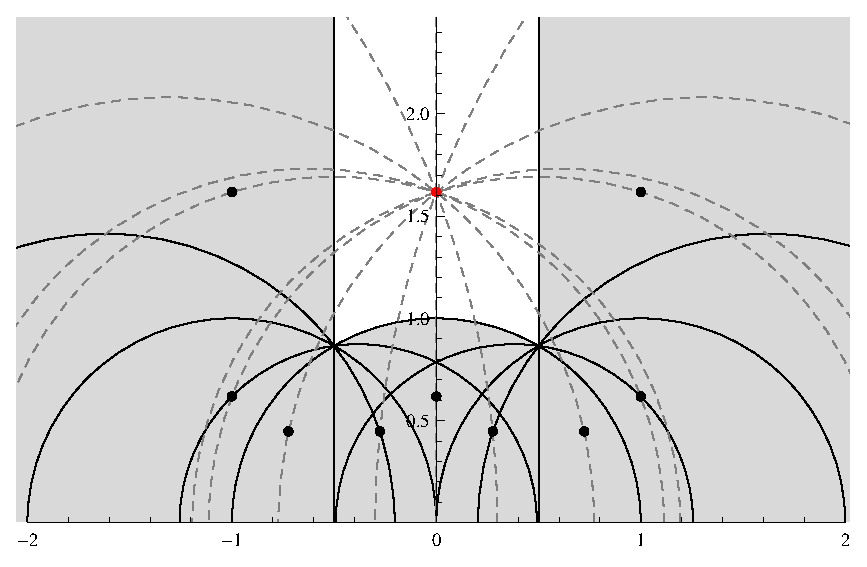
\includegraphics[width=\textwidth]{figures/normpoly-fundom-1}
\caption[The fundamental region $\FunDom$ as normal polygon]{The fundamental region $\FunDom$ can alternatively obtained by constructing the normal polygon with respect to a point $z$ on the imaginary axis with $\Im{z} > 1$. Above the point $z = \phi \ii$ (red) has been chosen, where $\phi = \frac{\sqrt{5}+1}{2}$ denotes the golden ratio.}
\label{fig_NormalPolyFunDom}
\end{figure}

\begin{figure}
\centering
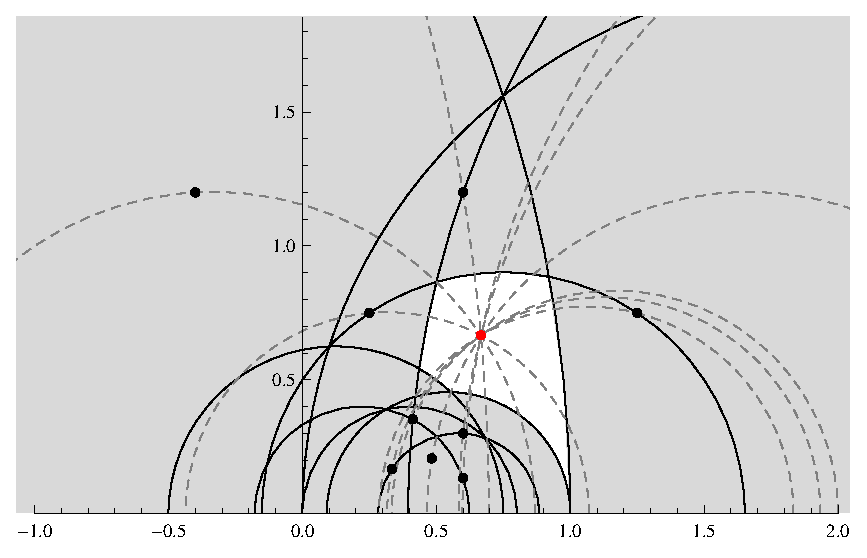
\includegraphics[width=\textwidth]{figures/normpoly-fundom-2}
\caption[An alternative fundamental region for $\PSL{\Z}$]{An alternative fundamental region for the action of $\PSL{\Z}$ on $\EU$. It is obtained by constructing the normal polygon for the point $\frac{2}{3}(1+\ii)$.}
\label{fig_AltNormalPolyFunDom}
\end{figure}

\begin{figure}
\centering
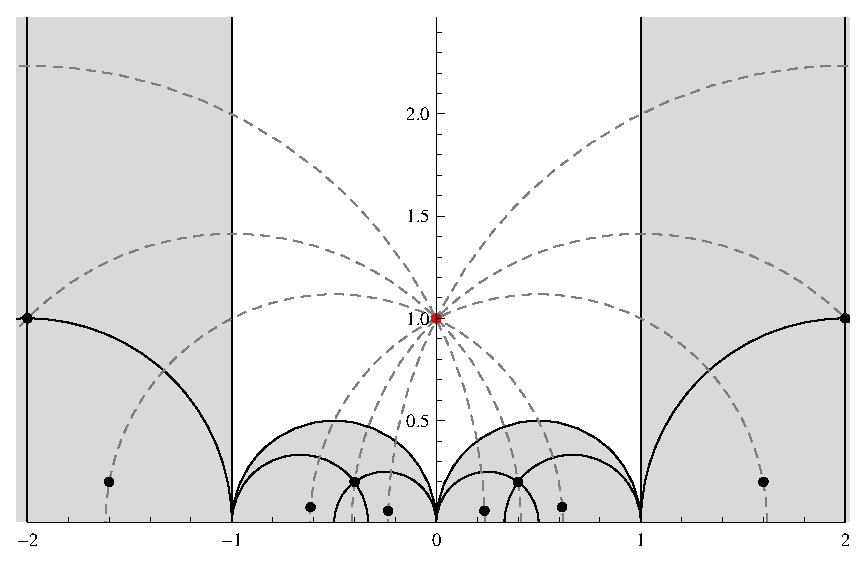
\includegraphics[width=\textwidth]{figures/normpoly-gamma2-1}
\caption[A fundamental region $\Gamma(2)$]{A fundamental region for the subgroup $\Gamma(2) \le \PSL{\Z}$. It is given by the normal polygon constructed with respect to the point $\ii$.}
\label{fig_Gamma2NormalPoly}
\end{figure}
